%-*- coding: utf-8 -*-
\section{一般的な麻雀のルール}
一般的な麻雀は図~\ref{hai}に示す34種類の牌がそれぞれ4枚,計136枚の牌を用いて4人で行うゲームである.牌は\textbf{\ruby{萬子}{まんず}},\textbf{\ruby{筒子}{ぴんず}},\textbf{\ruby{索子}{そうず}}と呼ばれる1から9の数字のいずれかが書かれた\textbf{数牌}と,文字が書かれた\textbf{字牌}がある.

ゲームは,\textbf{局}と呼ばれる単位に分割されている.局を特定の回数繰り返すことでゲームが終了する.それぞれの局で,プレイヤの1人が\textbf{親}という役割を担当し,その他のプレイヤが\textbf{子}という役割になる.局の始まりには,\textbf{山}と呼ばれる伏せられた牌の集合から,各プレイヤは13枚の牌を取る.山は伏せられているためプレイヤはどの牌を持ってくるかはわからない.プレイヤが所持する牌を\textbf{手牌}と呼び,他プレイヤには公開されない.山から1枚の牌を取り,14枚になった手牌の中から1枚の牌を場に捨てる行為を,親から順番に各プレイヤが繰り返して局は進行する.手牌が13枚のとき,山から取った牌または他プレイヤが捨てた牌を加えた14枚の牌の組み合わせが特定の条件を満たしていればプレイヤは上がり,点数を得ることができる.局は,山の残り牌数が特定数になるか,プレイヤの一人が上がったときに終了する.ゲームが終わったときの得点数で勝敗を競う.

同種の数牌が3連続している組を\textbf{\ruby{順子}{しゅんつ}},同一の牌が3枚の組を\textbf{\ruby{刻子}{こうつ}},同一の牌が2枚の組を\textbf{\ruby{雀頭}{じゃんとう}}と呼ぶ.順子,刻子,雀頭の例を図~\ref{syuntu},~\ref{koutu},~\ref{zyantou}に示す.順子と刻子を合わせて4つ,雀頭を1つの14枚の牌が上がりに必要な組み合わせである.図~\ref{agari}に上がりに必要な14枚の牌の組み合わせ例を示す.この14枚の組み合わせに\textbf{役}と呼ばれる特定のパターンがあるときが上がり条件となる.役の例として\textbf{\ruby{場風}{ばかぜ}}という役がある.この役は局ごとに定義される場風の牌の刻子が組み合わせに含まれているとき成立する.場風は東,南,西,北の4種類である.上がり点の要素となる\textbf{飜数}が,役に割り当てられている.役は複数存在し,役の種類により飜数が異なる.上がり時の組み合わせから,手牌の構成や上がり時の状況により計算される\textbf{符数}と呼ばれる値と,役による飜数を求め,その符数と飜数に応じて得られる上がり点が変動する.また,上がったプレイヤの役割が前述した親か子かによって,上がり点が変動する.
\if0 ゲーム中には場風と呼ばれるものが定義され,東場,南場,西場,北場がある.プレイヤには親と子が存在し,上がり点が異なる.\fi 
また,局の開始時に1種類の牌がドラとして指定され,この牌が上がったときの手牌に含まれているときにも,上がり点が変動する.麻雀では,手牌から上がりまでに最低限置き換えなければならない牌数を\textbf{\ruby{向聴数}{しゃんてんすう}},手牌に入れたとき向聴数が下がる牌を\textbf{有効牌}と呼ぶ.

\begin{figure}[p]
	\begin{center}
		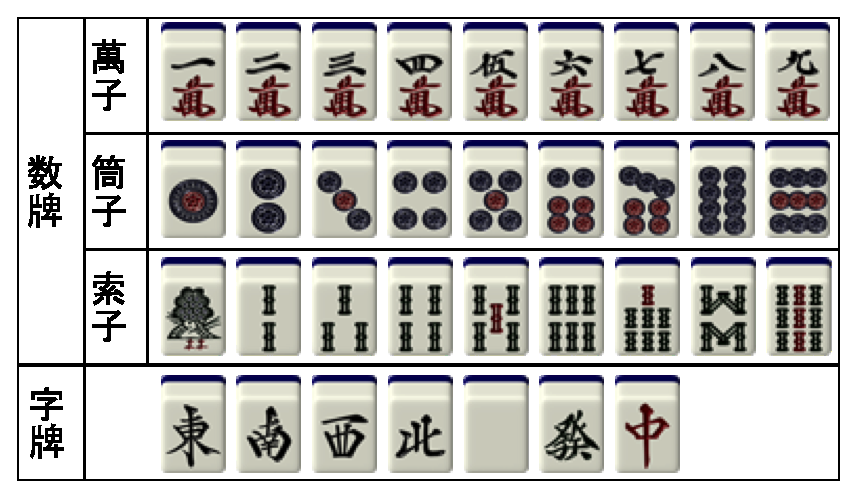
\includegraphics{fig/hai.eps}
	\end{center}
	\caption{牌の種類}
	\label{hai}

	\begin{center}
		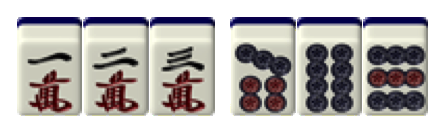
\includegraphics{fig/syuntu.eps}
	\end{center}
	\caption{順子の例}
	\label{syuntu}

	\begin{center}
		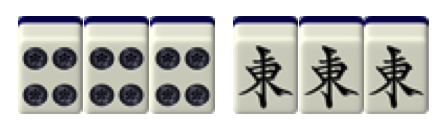
\includegraphics{fig/koutu.eps}
	\end{center}
	\caption{刻子の例}
	\label{koutu}

	\begin{center}
		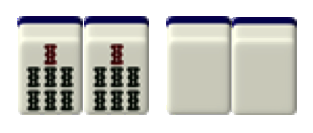
\includegraphics{fig/zyantou.eps}
	\end{center}
	\caption{雀頭の例}
	\label{zyantou}

	\begin{center}
		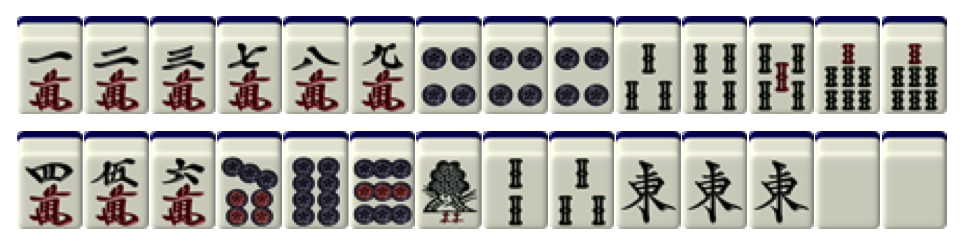
\includegraphics{fig/agari.eps}
	\end{center}
	\caption{上がりに必要な牌の組み合わせ例}
	\label{agari}
\end{figure}
%\clearpage

\section{一人麻雀のルール}
\if0 麻雀の多人数性を排除した一人麻雀を定義する.以下に一人麻雀のルールを説明する.\fi
他プレイヤを設定せず,不確定な情報のみを考慮する麻雀を一人麻雀と呼ぶ.一人麻雀とは以下のようなゲームである.
\begin{enumerate}
\item プレイヤは山から13枚の牌を取り,手牌とする.
\item プレイヤは山から1枚の牌を取り,手牌に加える.
\item 手牌が上がる条件を満たすならば,プレイヤは上がり点を得て,ゲームを終了する.
\item 手牌から牌を1枚捨てる.
\item 捨てた牌の枚数が18枚ならゲームを終了する.そうでないならば,2に戻る.
\end{enumerate}
2から4までの流れの単位を\textbf{巡}とする.ドラはランダムに1枚決める.一人麻雀の役を表~\ref{yaku}に,一人麻雀での点数表を~\ref{tensuu}に示す.役満は13飜固定となる.プレイヤは常に親,場風は東とする.

多人数の麻雀では,局1回は最初に上がれたプレイヤのみが点数を得ることができ,最終的にはゲーム終了時に最も点数が多いプレイヤの勝ちとなる.つまり,上がり率が高いこと,早く上がること,上がり点が高いことが重要である.一人麻雀においても,これらを目指す必要がある.

\begin{table}[p]
	\caption{一人麻雀で採用する役一覧}
	\label{yaku}
	\begin{center}
	 \begin{tabular}{|c|r|r|r|}
	 	\hline
	 	\textbf{役数} & \multicolumn{3}{|c|}{\textbf{役名}} \\ \hline
	 	1飜役 & 門前清自摸和 & 断幺九 & 平和 \\ \cline{2-4}
			  & 一盃口 & 役牌 & 場風 \\ \hline
	 	2飜役 & 三色同順 & 一気通貫 & 混全帯幺九 \\ \cline{2-4}
	 	      & 七対子 & 三暗刻 & 三色同刻 \\ \cline{2-4}
	 	      & 小三元 & & \\ \hline
	 	3飜役 & 混一色 & 純全帯幺九 & 二盃口 \\ \hline
	 	6飜役 & 清一色 & & \\ \hline
	 	役満   & 国士無双 & 四暗刻 & 大三元 \\ \cline{2-4}
	 	      & 字一色 & 大四喜 & 緑一色 \\ \cline{2-4}
	 	      & 清老頭 & 九蓮宝燈 & \\ \hline
		\end{tabular}
	\end{center}
\end{table}

\begin{table}[p]
	\caption{一人麻雀での点数表}
	\label{tensuu}
	\begin{center}
	 \begin{tabular}{|c|c|c|c|c|c|c|}
	 	\hline
	 	   & 20符 & 25符 & 30符 & 40符 & 50符 & 60符 \\ \hline
	 	1飜 & - & - & 1500 & 2000 & 2400 & 2900 \\ \hline
	 	2飜 & 2000 & 2400 & 2900 & 3900 & 4800 & 5800 \\ \hline
	 	3飜 & 3900 & 4800 & 5800 & 7700 & 9600 & 11600 \\ \hline
	 	4飜 & 7700 & 9600 & 11600 & \multicolumn{3}{|c|}{} \\ \cline{1-4}
	 	5飜 & \multicolumn{6}{|c|}{12000} \\ \hline
	 	6,7飜 & \multicolumn{6}{|c|}{18000} \\ \hline
	 	8,9,10飜 & \multicolumn{6}{|c|}{24000} \\ \hline
	 	11,12飜 & \multicolumn{6}{|c|}{36000} \\ \hline
	 	13飜〜 & \multicolumn{6}{|c|}{48000} \\ \hline
		\end{tabular}
	\end{center}
\end{table}